%%%%%%%%%%%%%%%%%%%%%%%%%%%%%%%%%%%%%%%%%%%%%%%%%%%%%%%%%%%%%%%%%%%%%%%%%%%%%%%%%%
\begin{frame}[fragile]\frametitle{}
\begin{center}
{\Large Costing}

{\tiny (Ref: Evaluating the Costs and Strategic Implications of Open-Source vs Commercial Large Language Models - Gopi Kirshna)}

\end{center}
\end{frame}

%%%%%%%%%%%%%%%%%%%%%%%%%%%%%%%%%%%%%%%%%%%%%%%%%%%%%%%%%%%%%%%%%%%%%%%%%%%%%%%%%%
\begin{frame}[fragile]\frametitle{}
\begin{center}
{\Large Open Source LLM Cost Considerations}
\end{center}
\end{frame}

%%%%%%%%%%%%%%%%%%%%%%%%%%%%%%%%%%%%%%%%%%%%%%%%%%%%%%%%%%%%%%%%%%%%%%%%%%%%%%%%%%
\begin{frame}[fragile]{Infrastructure Costs}
  \begin{itemize}
    \item High-performance GPU servers for on-premises: \$100,000+
    \item Cloud computing (monthly): \$10,000+
    \item Llama 2 usage cost: \$5/hour per machine
    \item Plan for at least 3 environments for AI deployment
  \end{itemize}
\end{frame}

%%%%%%%%%%%%%%%%%%%%%%%%%%%%%%%%%%%%%%%%%%%%%%%%%%%%%%%%%%%%%%%%%%%%%%%%%%%%%%%%%%
\begin{frame}[fragile]{Talent Expenses}
  \begin{itemize}
    \item Data scientists and ML engineers: \$150,000+ annual compensation
    \item Backend engineering and DevOps: \$100,000/year
  \end{itemize}
\end{frame}

%%%%%%%%%%%%%%%%%%%%%%%%%%%%%%%%%%%%%%%%%%%%%%%%%%%%%%%%%%%%%%%%%%%%%%%%%%%%%%%%%%
\begin{frame}[fragile]{Data Annotation}
  \begin{itemize}
    \item Annotation cost: \$100/hour
    \item Upfront bills for sizable datasets: \$100,000+
  \end{itemize}
\end{frame}

%%%%%%%%%%%%%%%%%%%%%%%%%%%%%%%%%%%%%%%%%%%%%%%%%%%%%%%%%%%%%%%%%%%%%%%%%%%%%%%%%%
\begin{frame}[fragile]{Energy and Cooling}
  \begin{itemize}
    \item Electricity bills (GPU on premises): \$10,000 - \$50,000/month
    \item HVAC investments: \$20,000+
  \end{itemize}
\end{frame}

%%%%%%%%%%%%%%%%%%%%%%%%%%%%%%%%%%%%%%%%%%%%%%%%%%%%%%%%%%%%%%%%%%%%%%%%%%%%%%%%%%
\begin{frame}[fragile]\frametitle{}
\begin{center}
{\Large Commercial API Cost Considerations}
\end{center}
\end{frame}

%%%%%%%%%%%%%%%%%%%%%%%%%%%%%%%%%%%%%%%%%%%%%%%%%%%%%%%%%%%%%%%%%%%%%%%%%%%%%%%%%%
\begin{frame}[fragile]{Usage-based pricing}
  \begin{itemize}
    \item OpenAI charges per API call
    \item Linear scaling with usage
    \item Consider volume discounts at scale
  \end{itemize}
  
\begin{center}
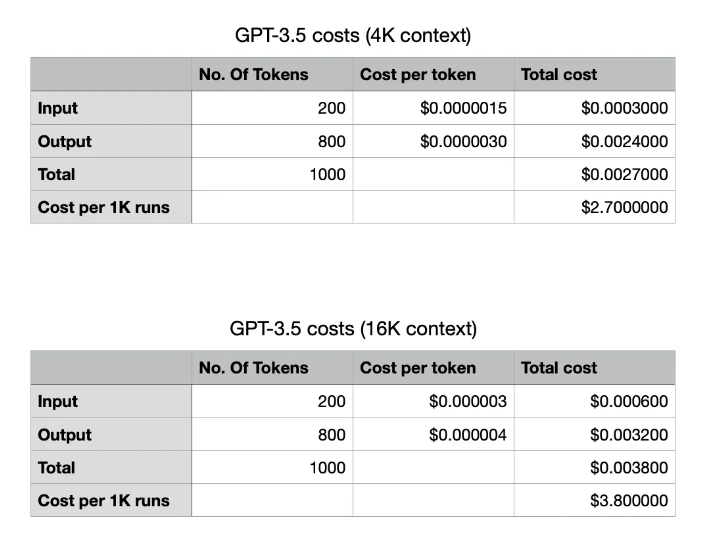
\includegraphics[width=0.6\linewidth,keepaspectratio]{llm103}


\end{center}	  
\end{frame}

%%%%%%%%%%%%%%%%%%%%%%%%%%%%%%%%%%%%%%%%%%%%%%%%%%%%%%%%%%%%%%%%%%%%%%%%%%%%%%%%%%
\begin{frame}[fragile]{Usage-based pricing}

\begin{center}
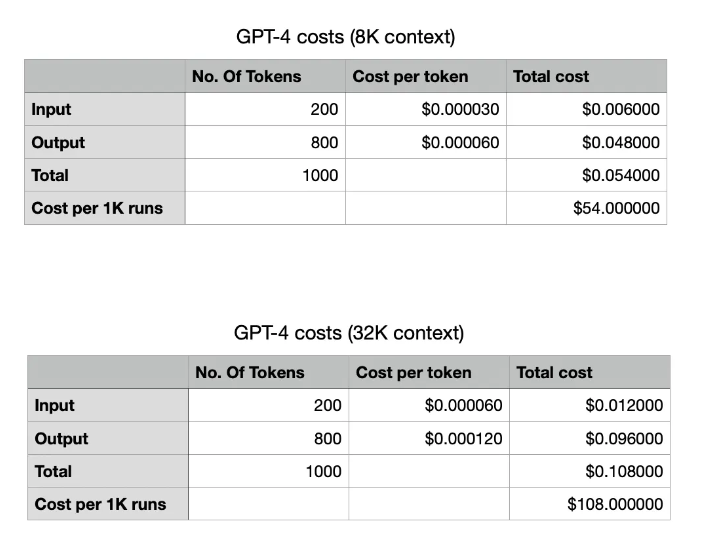
\includegraphics[width=0.6\linewidth,keepaspectratio]{llm104}
\end{center}	  
\end{frame}
%%%%%%%%%%%%%%%%%%%%%%%%%%%%%%%%%%%%%%%%%%%%%%%%%%%%%%%%%%%%%%%%%%%%%%%%%%%%%%%%%%
\begin{frame}[fragile]{Linear Pricing at Scale}
  \begin{itemize}
    \item Pricing increases significantly at scale.
    \item Linear pricing model as a justifiable cost line item.
    \item AI-driven cost reduction example: \$1 to 10c with GPT-4.
    \item Potential for volume discounts with OpenAI or Azure OpenAI.
  \end{itemize}
\end{frame}

%%%%%%%%%%%%%%%%%%%%%%%%%%%%%%%%%%%%%%%%%%%%%%%%%%%%%%%%%%%%%%%%%%%%%%%%%%%%%%%%%%
\begin{frame}[fragile]{Usage-Based Pricing Models}
  \begin{itemize}
    \item Models like Claude or PaLM follow usage-based pricing.
    \item Pay only for what you use, similar to Serverless compute.
    \item Ideal for experimentation and identifying impactful use cases.
    \item Contrast with upfront investment in private models and fine-tuning.
  \end{itemize}
\end{frame}

%%%%%%%%%%%%%%%%%%%%%%%%%%%%%%%%%%%%%%%%%%%%%%%%%%%%%%%%%%%%%%%%%%%%%%%%%%%%%%%%%%
\begin{frame}[fragile]{OpenAI Fine-Tuning}
  \begin{itemize}
    \item Fine-tuning cost: \$8 for 1000 conversations, each with 1000 tokens.
    \item Ongoing conversation cost: 1.5c per interaction.
    \item Cost-effective for relevance and training on company data.
  \end{itemize}
  
\begin{center}
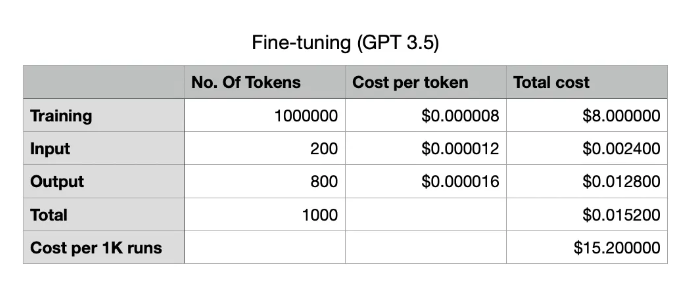
\includegraphics[width=\linewidth,keepaspectratio]{llm105}
\end{center}  
\end{frame}

%%%%%%%%%%%%%%%%%%%%%%%%%%%%%%%%%%%%%%%%%%%%%%%%%%%%%%%%%%%%%%%%%%%%%%%%%%%%%%%%%%
\begin{frame}[fragile]{Request Optimization}
  \begin{itemize}
    \item Optimize costs by caching responses and reducing API calls.
    \item Particularly effective for common and frequently asked queries.
  \end{itemize}
\end{frame}



%%%%%%%%%%%%%%%%%%%%%%%%%%%%%%%%%%%%%%%%%%%%%%%%%%%%%%%%%%%%%%%%%%%%%%%%%%%%%%%%%%
\begin{frame}[fragile]{Evaluating the Tradeoffs: Open Source vs. Commercial API}
  \begin{itemize}
    \item In-house AI expertise
    \item Data privacy policies
    \item Integration effort
    \item Model customization needs
    \item Cost of delays
    \item Growth trajectories
    \item Total cost of ownership
  \end{itemize}
\end{frame}

%%%%%%%%%%%%%%%%%%%%%%%%%%%%%%%%%%%%%%%%%%%%%%%%%%%%%%%%%%%%%%%%%%%%%%%%%%%%%%%%%%
\begin{frame}[fragile]{Best Practices for Cost Optimization}
  \begin{itemize}
    \item Well-scoped proof of concept
    \item Leverage cloud computing
    \item Understand right training data
    \item Consider smaller pretrained models
    \item Use batching and caching techniques
    \item Staged rollout and iterative enhancements
    \item Continuous monitoring of usage and spending
  \end{itemize}
\end{frame}

%%%%%%%%%%%%%%%%%%%%%%%%%%%%%%%%%%%%%%%%%%%%%%%%%%%%%%%%%%%%%%%%%%%%%%%%%%%%%%%%%%
\begin{frame}[fragile]{Key Takeaways for Senior Leaders}
  \begin{itemize}
    \item Weigh customization needs, integration complexity, data privacy, and in-house capabilities
    \item Factor in upfront infrastructure and talent investments for open source LLMs
    \item Account for cost growth with scaling usage for commercial LLMs
    \item Adopt a PoC approach and implement cost optimization best practices
    \item Avoid over provisioning during early stages
  \end{itemize}
\end{frame}

%%%%%%%%%%%%%%%%%%%%%%%%%%%%%%%%%%%%%%%%%%%%%%%%%%%%%%%%%%%%%%%%%%%%%%%%%%%%%%%%%%
\begin{frame}[fragile]{Summary}
  \begin{itemize}
    \item Open Source LLM: High initial costs, minimal ongoing costs
    \item Commercial API: Negligible startup costs, continuous spend with usage
    \item Strategic decisions based on organization's needs, priorities, and constraints
  \end{itemize}
\end{frame}

%%%%%%%%%%%%%%%%%%%%%%%%%%%%%%%%%%%%%%%%%%%%%%%%%%%%%%%%%%%%%%%%%%%%%%%%%%%%%%%%%%
\begin{frame}[fragile]\frametitle{}
\begin{center}
{\Large Costing}

{\tiny (Ref: 12 techniques to reduce your LLM API bill and launch blazingly fast products - Sahar Mor)}

\end{center}
\end{frame}

%%%%%%%%%%%%%%%%%%%%%%%%%%%%%%%%%%%%%%%%%%%%%%%%%%%%%%%%%%%%%%%%%%%%%%%%%%%%%%%%%%
\begin{frame}[fragile]\frametitle{Introduction}
    \begin{itemize}
        \item Open-ended language models gaining popularity in the last 12 months.
        \item Best practices for managing cost, latency, and accuracy are evolving.
        \item Minimal latency and cost are crucial for user-facing applications.
        \item 2024 marks the transition of LLM apps to production-ready scalable applications.
    \end{itemize}
\end{frame}

%%%%%%%%%%%%%%%%%%%%%%%%%%%%%%%%%%%%%%%%%%%%%%%%%%%%%%%%%%%%%%%%%%%%%%%%%%%%%%%%%%
\begin{frame}[fragile]\frametitle{Semantic Caching}
    \begin{itemize}
        \item Caching stores prompts and responses for future use.
        \item Exact match or similar match prompts can utilize cached responses.
        \item Benefits:
            \begin{itemize}
                \item Faster and cheaper inference in production.
                \item Faster development cycles.
                \item Simplifies fine-tuning by using stored prompt-response pairs.
            \end{itemize}
        \item Refresh the cache periodically to prevent outdated responses.
    \end{itemize}
\end{frame}

%%%%%%%%%%%%%%%%%%%%%%%%%%%%%%%%%%%%%%%%%%%%%%%%%%%%%%%%%%%%%%%%%%%%%%%%%%%%%%%%%%
\begin{frame}[fragile]\frametitle{Summarizing Lengthy Conversations}
    \begin{itemize}
        \item Multi-turn conversations can accumulate redundant text.
        \item Summarize conversations to remove fluffy parts and reduce tokens.
        \item Use tools like LangChain’s ConversationSummaryMemory or GPT-3 Turbo for summarization.
        \item ConversationBufferWindowMemory retains the last X interactions.
        \item Summarization saves tokens and reduces latency.
    \end{itemize}
\end{frame}

%%%%%%%%%%%%%%%%%%%%%%%%%%%%%%%%%%%%%%%%%%%%%%%%%%%%%%%%%%%%%%%%%%%%%%%%%%%%%%%%%%
\begin{frame}[fragile]\frametitle{Compressing Prompts}
    \begin{itemize}
        \item Lengthy prompts lead to slow and expensive LLM API calls.
        \item Use LangChain’s ConversationSummaryMemory to compress prompts.
        \item Longer context windows and advanced prompting techniques can be problematic.
        \item Improving context retrieval for RAG-powered apps is crucial.
        \item Routing to cheaper models and accelerating inference can also enhance performance.
    \end{itemize}
\end{frame}

%%%%%%%%%%%%%%%%%%%%%%%%%%%%%%%%%%%%%%%%%%%%%%%%%%%%%%%%%%%%%%%%%%%%%%%%%%%%%%%%%%
\begin{frame}[fragile]\frametitle{Improving Context Retrieval for RAG}
    \begin{itemize}
        \item Refine retrieval mechanism for sharper, cost-effective results.
        \item Ensure only relevant context is retrieved and sent to the LLM.
    \end{itemize}
\end{frame}

%%%%%%%%%%%%%%%%%%%%%%%%%%%%%%%%%%%%%%%%%%%%%%%%%%%%%%%%%%%%%%%%%%%%%%%%%%%%%%%%%%
\begin{frame}[fragile]\frametitle{Routing to Cheaper Models}
    \begin{itemize}
        \item GPT-4 is 8x more expensive than Claude 2.1.
        \item Use inferior models for tasks that don't require high-end models.
        \item Open-source packages like LiteLLM make the transition seamless.
    \end{itemize}
\end{frame}

%%%%%%%%%%%%%%%%%%%%%%%%%%%%%%%%%%%%%%%%%%%%%%%%%%%%%%%%%%%%%%%%%%%%%%%%%%%%%%%%%%
\begin{frame}[fragile]\frametitle{Accelerating Inference}
    \begin{itemize}
        \item Packages like vLLM and Hugging Face's TGI speed up open-source language models.
        \item Support models like Llama 2, Mixtral-8x7B, and Phi 2 out of the box.
    \end{itemize}
\end{frame}